\documentclass{article}

\usepackage{siunitx} % Provides the \SI{}{} and \si{} command for typesetting SI units

\usepackage{graphicx} % Required for the inclusion of images

\usepackage{tabularx} % Tables

\usepackage{natbib} % Required to change bibliography style to APA

\usepackage{amsmath} % Required for some math elements

\usepackage{parskip} % Formatting

\usepackage{tikz}
\usetikzlibrary{automata,positioning} %for nodes

% Many options for pseudocode
\usepackage{algorithm2e}
\usepackage{algorithmic}

\usepackage[demo]{graphicx}
\usepackage{caption}
\usepackage{subcaption}

\usepackage{listings} % Python code blocks

\setlength\parindent{0pt} % Removes all indentation from paragraphs

\title{Lab 3 Report: Wall Follower} % Title

\author{Team 4 \\\\ Rohan Wagh \\ Oliver Rayner \\ Gabriel Jimenez \\ Kairo Morton \\\\ 6.4200/16.405: Robotics Science and Systems} % Team # + Names, Class (RSS)

\date{\today} % Date for the report

\begin{document}

\maketitle

\section{Introduction}
In lab 3, group 4 designed a safety controller component to run alongside our wall follower package that was ported to run on the RSS racecar platform.

This work marked the first steps towards implementing an autonomous system, as we were able to take the semantic description of a goal (i.e. follow the wall without crashing), and deploy the necessary components so that autonomous execution achieves that goal. In terms of specific deliverables for Lab 3 we had to log into the physical car from our local machines, and use teleop with the controller to manually drive the car. From there we deployed our code on the racecar, and continued to iterate on the implementation until it was able to achieve the autonomous execution goals of wall following and collision failsafe.

For tackling the wall follower porting task we tested how various of our existing wall follower implementations performed, and were able to achieve the desired behavior after minor tweaks to the best performing one. As for our solution to the safety component for avoiding collisions, we built upon our concept of defining laser scan data sections in order to define a bounding box safety zone where an infringing range signal would trigger an immediate stop.

\section{Technical Approach}

\subsection{Distance-Based Wall Follower}
The motivation for this version of the wall follower is to control the robot based on an error signal describing the deviation from the desired distance from the wall: simply calculated as the current distance - desired distance. This error feeds into a PID controller, which determines the ideal corrective steering angle to keep the robot on course. 

\subsubsection{Parsing Laser Scan Input}
At a high level, the wall follow program functions by taking in a laserscan and commanding the robot to drive at an appropriate turning angle and speed. The wall follower program begins by taking the data from the laser scan topic and parsing it into two regions of interest around the car: front and side. 

\begin{figure}[h]
\begin{center}
\includegraphics[width=0.65\textwidth]{LaserScan.png} % Include the image placeholder.png
\caption{Laser Scan range partitioning for distance-based wall follower}
\end{center}
\end{figure}

The front region of interest is directly in front of the car and focuses on identifying inside corners. If there is any object detected within desired distance $+$ turning radius of the car the node will publish a turning command instructing the car to take a sharp turn away from the wall. This allows the car to effectively handle inside corners and end the turn near the appropriate distance from the new wall. 

The side region is all points within 90 degrees to 45 degrees of the car’s wall-following side. This region’s range can be adjusted using parameters and allows the wall follower to be modified or calibrated based on the performance of the physical robot. These points are used to estimate the wall position and calculate an error value for the control. 

\subsubsection{Wall Estimation}
The points from the laser scan are converted from polar coordinates to cartesian coordinates and fed to NumPy’s polyfit function. This function returns constants describing a linear line of best fit, which in this context represents a line describing the wall’s location with respect to the laser frame. Since the laser frame is superimposed on the robot’s frame, we did not need to use a coordinate transfer on the line. 

\begin{figure}[h]
\begin{center}
\includegraphics[width=0.65\textwidth]{WallEstimation.png} % Include the image placeholder.png
\caption{Wall estimation visualization }
\end{center}
\end{figure}

Once the line’s describing line is calculated, the distance between the robot and the wall is calculated using the formula for the orthogonal distance of a linear line from the origin: in this context, the origin is the robot’s location. This calculated distance is then used to find the error, as current distance - desired distance.

\subsubsection{PID Control}
The last step in wall following is to pass this error into the PID controller. This controller is initialized at the start of the program and keeps track of derivative and integral errors over time. The PID controller was designed as a separate class and contains “update” and “get\_drive” functions. Once the error is calculated, the update function is used to find new values for the derivative and integral error. The get\_drive function is then called to get the new turning angle for the car based on the current error, derivative error, and integral error. This is then used to set the drive topic and move the car. 

\subsection{High Level Organization}
One of the key motivations for this wall-follow program was being able to catch the wall from unideal initial positions. This may include, for example, the robot facing away from a wall or starting in the opposite direction. 

\begin{figure}[h]
\begin{center}
\includegraphics[width=0.65\textwidth]{Unideal.png} % Include the image placeholder.png
\caption{Example unideal starting location}
\end{center}
\end{figure}

In these scenarios, the robot was not be able to correct itself using the PID control loop and a state machine was developed to handle these cases. The state machine has three states: “LOOKING,” “MOVING,” and “LOCKED.” Upon initialization, the robot begins in the “LOOKING” state and will not begin wall following until it reaches the “MOVING” state.

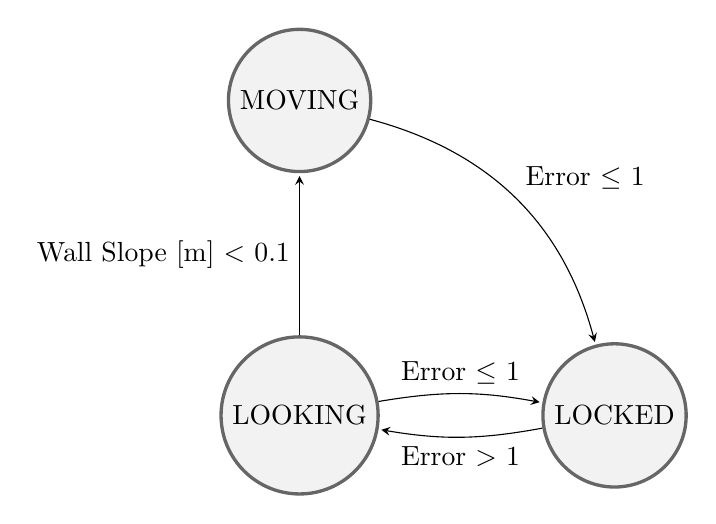
\begin{tikzpicture}%
  [>=stealth,
   shorten >=1pt,
   node distance=4cm,
   on grid,
   auto,
   every state/.style={draw=black!60, fill=black!5, very thick}
  ]
\node[state] (mid)                  {LOOKING};
\node[state] (upper) [above=of mid] {MOVING};
\node[state] (right) [right=of mid] {LOCKED};

\path[->]
%   FROM       BEND/LOOP           POSITION OF LABEL   LABEL   TO
   (upper) edge[bend left]     node                      {Error $\leq$ 1} (right)
   (mid)   edge[bend left=10]  node                      {Error $\leq$ 1} (right)
           edge                node                      {Wall Slope [m] $<$ 0.1} (upper)
   (right) edge[bend left=10]  node                      {Error $>$ 1} (mid)
   ;
\end{tikzpicture}

\subsubsection{Looking State}
This state describes the robot being unattached to a wall. In this state, the robot will move at an angled path and look for parallel wall segments on the appropriate side. Once the wall estimation returns a wall found with a slope close to 0, meaning close to parallel on the appropriate side, the state changes to “MOVING.” Alternatively, if the error is under 1 meter, the state moves to “LOCKED.”

\subsubsection{Moving State}
The moving state starts the PID control and begins to follow this found wall. Once the error reaches under the desired distance, the state is then switched to “LOCKED.”

\subsubsection{Locked State}
This state also runs the PID control. The only exit from this state is if the error jumps to over the desired distance in length, this indicates that the robot has strayed from the wall or an outside corner is encountered. In both of these cases, the best thing for the robot to do is turn until it finds the wall again. Thus, if the error jumps to over 1 meter, the state switches back to “LOOKING.”

\pagebreak
\section{Experimental Evaluation}

Our wall following and crash avoidance (safety controller) software was thoroughly tested on the “racecar” platform to ensure robustness in a variety of conditions. As such, we evaluated the performance of our method qualitatively in various real world scenarios. Through the qualitative assessment, we observed our method to be robust to multiple wall geometries, velocity settings and turn types. In addition, it is seen through our tests that the crash avoidance system can handle different object types and responds rapidly to stop forward motion of the “racecar” platform. In this section, we detail the specifics of the tests run to evaluate the performance of our method. 

\subsection{Qualitative Observation and Testing}
We ran the robot in a series of varying environments to qualitatively evaluate the performance. Pictured below are examples of turn types with the orientation keyword - inside or outside corners - that will be used throughout the evaluation. 

\begin{figure}[h]
\centering
\begin{subfigure}{.5\textwidth}
  \centering
  \includegraphics[width=.4\linewidth]{InsideCorner.png}
  \caption{Inside corner example}
  \label{fig:sub1}
\end{subfigure}%
\begin{subfigure}{.5\textwidth}
  \centering
  \includegraphics[width=.4\linewidth]{OutsideCorner.png}
  \caption{Outside corner example}
  \label{fig:sub2}
\end{subfigure}
\caption{Types of corners tested}
\label{fig:test}
\end{figure}

\subsubsection{Handling Various Wall Geometries}
We first evaluated our system on walls with flat surface geometry void of any special features. In doing so, we were able to isolate and thus solely evaluate the ability of the wall following algorithm to maintain a set distance of 0.25 meters from the wall. During this test we observed the “racecar” making very few corrections to its orientation and distance from the wall once the setpoint distance was reached. This desirable behavior can be attributed to the well-tuned proportional and derivative control constants which enabled the system to make adjustments to its position while dampening high-frequency oscillations in the control signal. In addition, to flat wall geometries, we also tested the system on the wall with protruding and inset features. 

\pagebreak
\begin{figure}[h]
\centering
\begin{subfigure}{.5\textwidth}
  \centering
  \includegraphics[width=.6\linewidth]{Protruding.png}
  \caption{Protruding feature}
  \label{fig:sub1}
\end{subfigure}%
\begin{subfigure}{.5\textwidth}
  \centering
  \includegraphics[width=.6\linewidth]{Inset.png}
  \caption{inset feature}
  \label{fig:sub2}
\end{subfigure}
\caption{Examples of protruding of inset features}
\label{fig:test}
\end{figure}

In both of these cases, we observe similar performance to the baseline flat wall tests however, due to the robot having to navigate around these features the desired parallel orientation to the wall is occasionally lost earlier than expected in favor of a heading that points more in the direction of the wall directly after the feature. We believe this to be due to the linear regression algorithm to detect the wall’s position and orientation being run over a portion of the LiDAR scan which contains points corresponding to locations before and after the special wall feature. This results in a line to follow that is a weighted average of the two lines representing the walls before and after the inset or protruding feature. Nonetheless, our system is robust to these different wall geometries and continues to follow the wall as expected after handling any special features gracefully.   

\subsubsection{Handling Turn Types and Angles}
In addition to straight driving, we also evaluated our system’s ability to handle various turns and corners. We classify corners into two distinct categories: inside and outside corners. See Figure 4 for examples of both corner types. Our system was evaluated on both types of corners with various required turn angles. From these tests, we observed smooth motion around all types of corners even for more extreme turn angles. 

\begin{figure}[h]
\centering
\begin{subfigure}{.5\textwidth}
  \centering
  \includegraphics[width=.6\linewidth]{TightInside.png}
  \caption{Extreme inside corner}
  \label{fig:sub1}
\end{subfigure}%
\begin{subfigure}{.5\textwidth}
  \centering
  \includegraphics[width=.6\linewidth]{TightOutside.png}
  \caption{Extreme outside corner}
  \label{fig:sub2}
\end{subfigure}
\caption{Examples of extreme turn angles}
\label{fig:test}
\end{figure}

\pagebreak
We hypothesize the positive performance on inside corners to be due to the lookahead wall detection and our well-tuned responsive PD controller. Finally, our system's ability to handle outside corners with large turn angles is due to the underlying state machine that transitions to the “Looking State” after the end of the current wall in order to find the next wall to follow. 

\subsubsection{Handling Multiple Speeds}
 To further evaluate the possible failure modes and overall robustness of our method we ran the experiments detailed in parts 1) and 2) above at speeds of both 0.5 m/s and 1 m/s. We observed that at both speeds the performance detailed above is of the same quality even though the “racecar” must react faster and more precisely to any changes in the environment at higher speeds.  The robustness of the wall following algorithm to changes in velocity can be attributed to the well-tuned PD controller and the forward-looking wall detection algorithm which allows the system to recognize wall features such as corners early and react accordingly. 

 \subsubsection{Crash Avoidance/Safety}
 We qualitatively evaluated our safety controller using the standard red paper block obstacle and with pedestrian insertion into the robot path. In both of these cases, the safety controller stopped the robot quickly within the defined front and side thresholds. Thus, allowing us to test our system thoroughly without fear of damaging the “racecar” platform or injuring any pedestrians. 

 \begin{figure}[h]
\begin{center}
\includegraphics[width=0.65\textwidth]{SafeRobot.png} % Include the image placeholder.png
\caption{Robot stopping in front of obstacle}
\end{center}
\end{figure}

\subsection{Evaluation Takeaways}
All in all, by evaluating our wall following software and safety controller in a plethora of contrived and real world scenarios we can be confident in the robustness of our algorithms as well as the overall performance of our system.

\pagebreak
\section{Conclusion}
Through Lab 3, Group 4 managed to complete all deliverables by successfully deploying the improved wall follower code and the newly implemented safety controller that stops the car upon detecting an imminent collision. The wall follower component required minimal changes, thus the bulk of the development work was spent on the safety controller bounding box implementation, as well as exploring options to achieve better performance.

\section{Lessons Learned}

\subsection{Rohan Wagh}
This lab was extremely engaging and satisfying to complete. After working on the simulated robot and environment, I was excited to get to work on the physical robot itself. One of the interesting takeaways from this lab was how different theory and practice can be. As we developed the wall follower and safety controller, many things that worked in the rviz simulation were not as successful in the physical robot. Besides technical learning, this lab also served as a great way to get accustomed to the team environment. As a whole, team 4 is a well-gelled group. Everyone on the team was excited to work on the robot and looked to contribute in any way possible. In addition, we setup strong communication lines - messenger chats for our team and pod - which helped coordinate time, deliverables, and status throughout the lab. In addition, we were able to split responsibilities for the report, presentation, and lab evenly and in a way where each team member was involved and equally contributing. The one spot fo improvement is in our communication with other teams in our pod. At times, we were searching for the robot and unable to get in contact with the team that had possession of the robot. At the same time, we did not communicate well with our other pod mates about when to hand off the robot after we completed the lab, which led to some confusion about handoff. Looking back, we could have been better communicators with the other teams in the pod and will work to improve that for next week. Overall, this lab experience was rewarding and I look forward to working with the team and robot in the future. 

\subsection{Gabriel Jimenez}
Throughout Lab 3 a main personal takeaway from a technical standpoint was that the best approach can be the simple solution. By overcomplicating my wall follower logic, I ended up with a worse solution as a result of creating more edge cases that then worsened the desired wall following behavior metric. As for communication and collaboration lessons, I would say that my experience during Lab 3 has validated my approach of direct and open communication, with clear central documentation of outstanding tasks and assignments. We had little friction in terms of dividing the required technical and communication work amongst the team members.

\subsection{Kairo Morton}
This lab more than a technical exercise was a lesson in communication, teamwork and planning. While all of us had solved the wall following problem in simulation, it was unclear whose solution would work in practice on the real robotics platform. By giving everyone's code and ideas a chance to be tested on the robot we were able to quickly find that Rohan's code produced the best results in practice with minimal modifications. After this discovery, the rest of this lab focused on setting up communication channels, getting to know each other and planning tests to evaluate and ultimately report the performance of our system. Through this process I originally found it challenging to work on a team of this size with many valid ideas and possible solutions to problems. However, the more we worked together the better we were able to build trust in each other's abilities which ultimately made decision making and comprimise easier. All in all, this lab allowed us to truly go from individuals to a collective group that can effectively solve problems, technical and otherwise. 



\end{document}
